\documentclass{report}
\usepackage{setspace}
\doublespacing
\usepackage[utf8]{inputenc}
\usepackage{graphicx}
\usepackage{amsmath}
\usepackage{indentfirst}
\usepackage[labelfont=bf]{caption}

\title{Polyphase Filter Banks: A Physicist's Attempt}
\author{Matthew Cooper}
\date{Sometime in May, 2019}
\begin{document}
\maketitle

\tableofcontents{}

\newpage
\chapter{Introduction}

In the modern era, the speed of digital processing components has made it such that the gap between digital and analog is becoming ever smaller, allowing us the advantages that come with conversion of analog signals to digital signals.  These advantages are numerous, but, as with anything, there is an equivalent exchange, and there are tradeoffs in using digital signals which, if not taken into account, can turn a scientific data product into something completely unusable.

In my researching of this subject, it became clear early on that my understanding of the fundamentals that go into digital signal processing (DSP hereafter) were not up to par, which resulted in several hours of researching different aspects of DSP in order to complete the mental picture I needed.  It is my goal in the pages of this report to recreate, as best I can, this journey, making pitstops at different ideas that helped shape my current, albeit incomplete understanding.  

The first reference I was able to find for polyphase filter bank implementation was a paper from 1973 (Schafer and Rabiner, 1973).  In this paper, however, the term polyphase had not been coined yet.  Its original implementation was to increase resolution of frequency channels for speech analysis and synthesis.  Not suprising, this came out of Bell Labs.  We'll discuss this paper in greater detail when we come to the theory side of things.

Although it started as a method of reconstructing speech output, the applications of polyphase filter banks has found use in almost all areas where channelization is required, such as cell phone signal downconversion and up conversion (Harris, 2003), as well as being considered for implementation in the Extended Owens Valley Solar Array(CITE).  

In this report, we will review some basics of analog-to-digital conversion, methods which have been created to navigate the restrictions that such conversions place on the type of data which can be sampled, and then proceed with how polyphase filter banks are utilized in the optimization of such a process.  

\chapter{Fundamentals of Digital Signals}
\section{Analog Vs. Digital}

The filtering and manipulation of analog signals has been widely used for decades.  Why, then, is there the push for analog-to-digital conversion?  For systems where the average power of a signal is the only necessity, staying in the analog domain is perfectly acceptable.  The issue arises when a system also needs to accurately measure and record phase information.  In analog systems, the gain to phase balance of a signal cannot be maintained to better than $1\%$ over a range of temperatures (Harris, 2003).  This is particularily crippling for a multi-antennae radio array, which relies on phase-locking between antennae in order to steer the beam.  Since no two antennae's analog components can match identically, leaving the signal in the analog domain can produce spurious phase shifts, which are functions of many variables which cannot be accounted for simply, if at all.  This is where analog-to-digital conversion is helpful, since the phase information stored in a digital signal is not subject to environmental effects.  

\section{Analog Signal Sampling}

In analog-to-digital conversion, there are two relations which must be considered: the Nyquist Sampling Theorem, and the Frequency Resolution Relation.  These combined determine the sampling rate which must be attained in order to recover a maximum frequency, as well as how much resolution there will be between frequencies.  The Nyquist Theorem (Landau, 1967) states that
\begin{equation}
f_{crit} = \frac{f_{sample}}{2}
\end{equation}

where $f_{crit}$ is the maximum frequency which can have power 'definitively' attributed to it (i.e. has no alias), and $f_{sample}$ is the sampling frequency.  This relation is troubling for radio transmissions.  Consider a 10 GHz signal.  In order to recover this signal, it must be sampled at 20 billion samples per second.  At 64 bit resolution, this equates to around 160 Gigabytes of data.  Currently, FPGA's on the market sit in the MHz processing speed range, although ADC converters currently exist which can handle giga-samples per second.

The second relation, the Frequency Resolution Relation, gives a size requirement for the hardware register which must be fed to the FFT in order to maintain a specific resolution between frequencies.
\begin{equation}
f_{res} = \frac{f_{sample}}{N}
\end{equation}

where $f_{res}$ is the resolvability.  So, for higher sample rates, the register size must also increase to maintain frequency resolvability.  Clearly, a register which is of the order of 160 Gigabytes is something science fiction would hesitate to create, so how is this issue circumvented? The obvious answer is to sample less, but therein lies the problem, since in the process we lose information either by loss of resolution or by ambiguity in frequency aliasing.  The method which was created to circumvent this problem was the concept of downconversion.

\section{Downconversion}

Downconversion (heterodyning) was originally worked on by Nikola Telsa and Reginald Fessenden (Espenschied 1959).  Fessenden patented the heterodyne principle in 1902, and that same year founded the National Electrical Signaling Company (NESCO).  John Vincent Lawless Hogan, who went to work for Fessenden in 1910, showed how the concept had greatly improved the sensitivity of radio receivers (Godara, 1999).  The introduction of this concept revolutionized electromagnetic signaling, and it is no stretch to say that without it, the subject of this paper, as well as many other DSP related ideas, would never have existed.

What is heterodying? Heterodyning is the process by which a signal is mixed with a higher frequency signal in order to mirror the signal to a lower frequency band.  This can be easily shown mathematically.  Consider a monochromatic input signal, $x_{in}$, and a local signal, $x_{lo}$.  Then,
\begin{align}
x_{in}*x_{lo}& = sin(f_{in}t)sin(f_{lo}*t)\\
             & = \frac{1}{2}[cos((f_{lo}-f_{in})*t) - cos((f_{lo}+f_{in})*t]
\end{align}

Here, we see that there are two mirrors of the input signal; one which is at higher frequencies, and one which is at lower frequencies, with an example shown in Figure 1.  
\begin{figure}[ht]
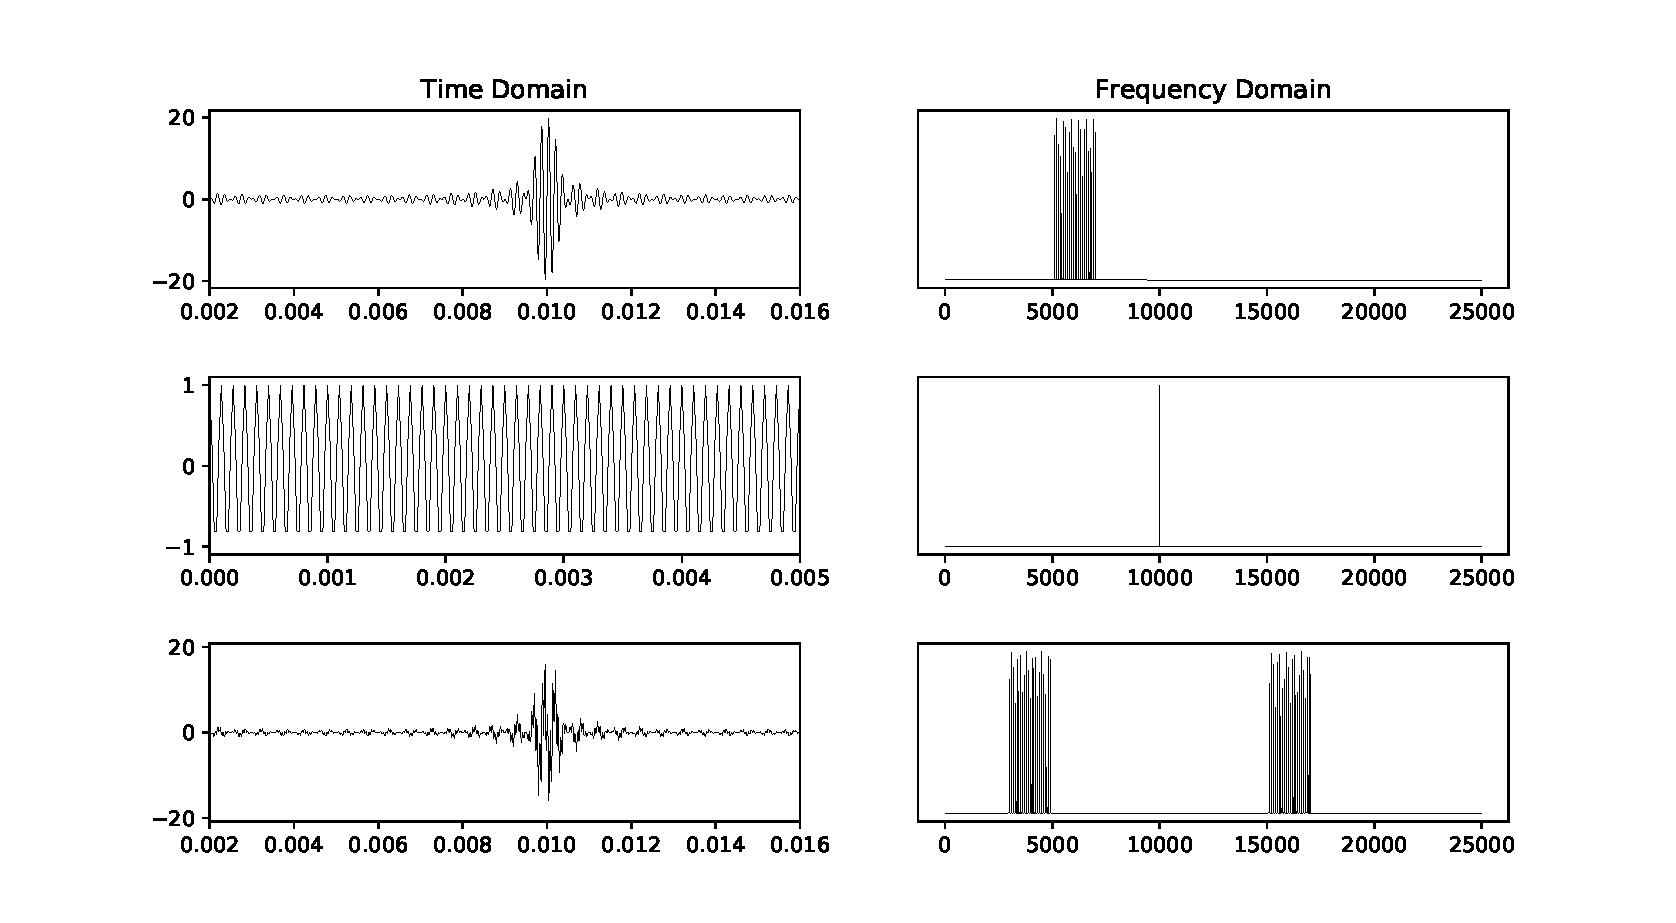
\includegraphics[scale=.45]{Figure_1.pdf}
\caption{(top) Signal $x_{in}$ in the time and frequency domain (middle) Signal $x_{lo}$ in time and frequency domain (bottom) Signal $x_{in}x_{lo}$ in the time and frequency domain}
\end{figure}

The part we are interested in is, of course, the lower frequencies, since we don't have to sample these as often.  Therefore, the higher frequency components must be removed.  We remove these signal contributions by the process of filtering.

\section{Digital Signal Filters}

Digital signal filters are arguably one of the biggest fields within the realm of electrical engineering, and for good reason.  This process allows one to attenuate certain frequency bands, while leaving others (relatively) unaffected. 

\begin{figure}[ht]
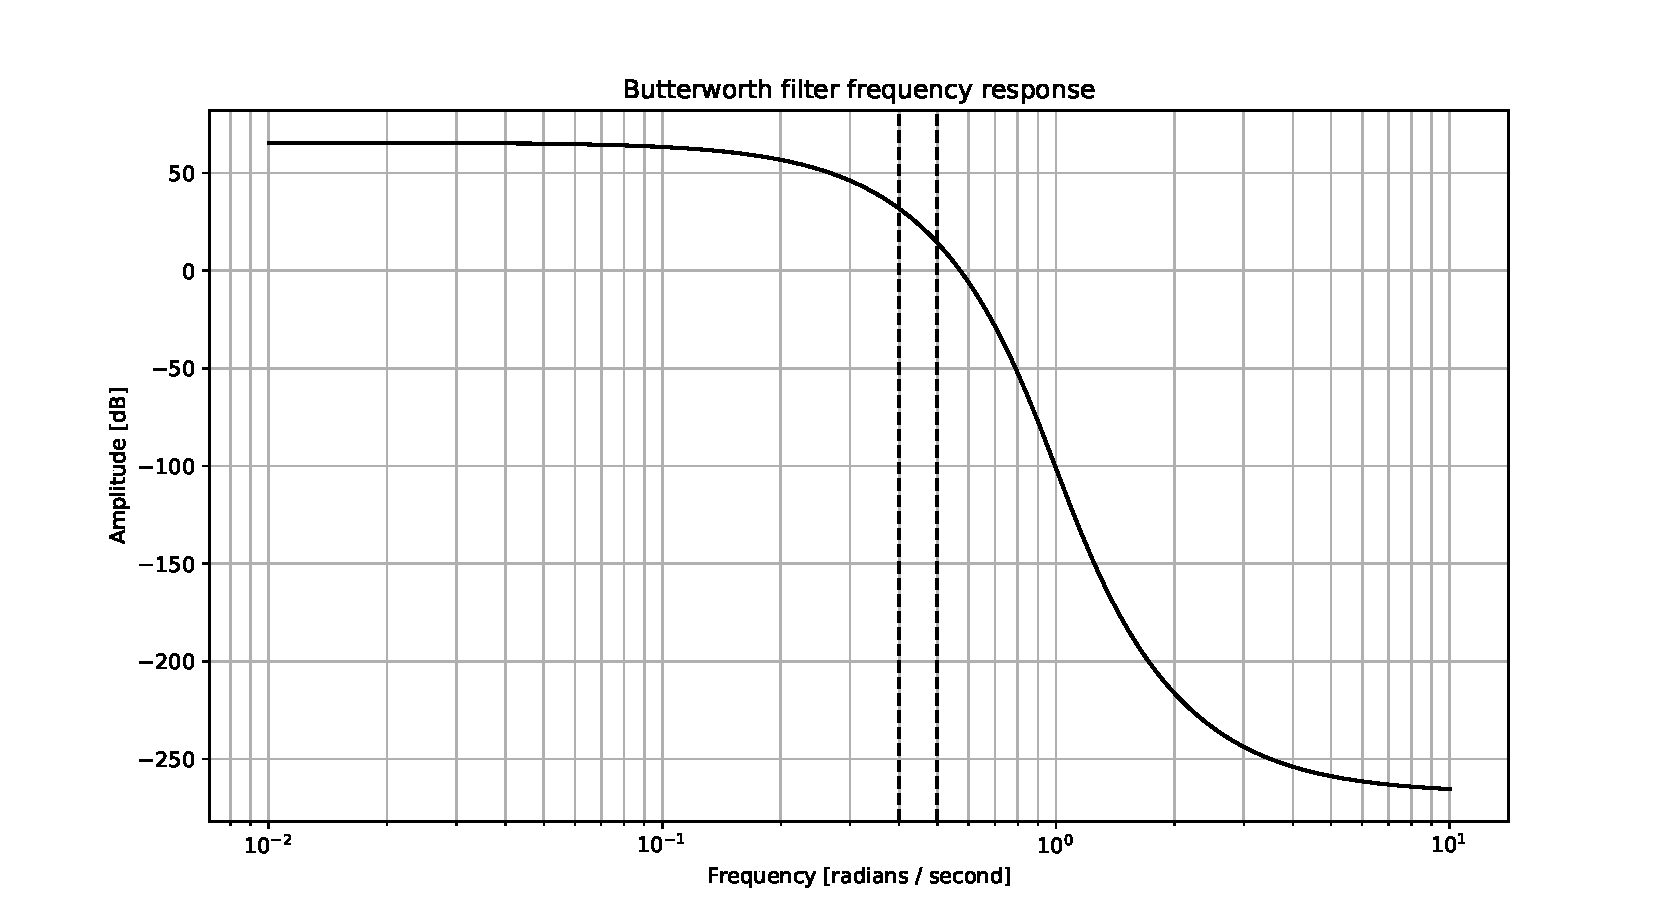
\includegraphics[scale=.45]{Figure_2.pdf}
\caption{Plotted above is the frequency responses for a Butterworth filter of low-pass type.  The y-axis indicated the attenuation (in dB) of the different frequency components.  The first dashed line indicated the end of the pass-band, and the second is the beginning of the stop band.}
\end{figure} 

Figure 2.1 shows a typical frequency response profile for a filter transfer function.  As can be seen, all frequencies are affected, but the stopband frequences are attenuated much more heavily than in the passband.  Other filter types, such as Chebyshev, Bessel, and Elliptic, have other features which would appear in such a plot.  The Butterworth filter has no rippling in the attenuation of its passband, whereas an Elliptic or Bessel filter would.  Thus, different filters are chosen for different applications.  Specific bandstop filters have been created for radio astronomy in particular, such as the cryogenic S-band filter, which is a hardware bandstop filter which mimics a Chebyshev/Elliptic bandpass filter (Srikanta, 2012).

Signal filters are commonly derived in the Laplace domain, due to the simplicity of the mathematics.  The task is then to convert it to the Z-domain, via transforms such as a bilinear transform.  One then takes the impulse response of a given filter, which for an FIR filter gives the coefficients with which to convolve the input signal, via.
\begin{equation}
y[n] = \sum^{N-1}_{k=0}x[k]h[n-k]
\end{equation}
Example time-domain coefficients for the Butterworth filter above are given in Figure 2.2.  

\begin{figure}[ht]
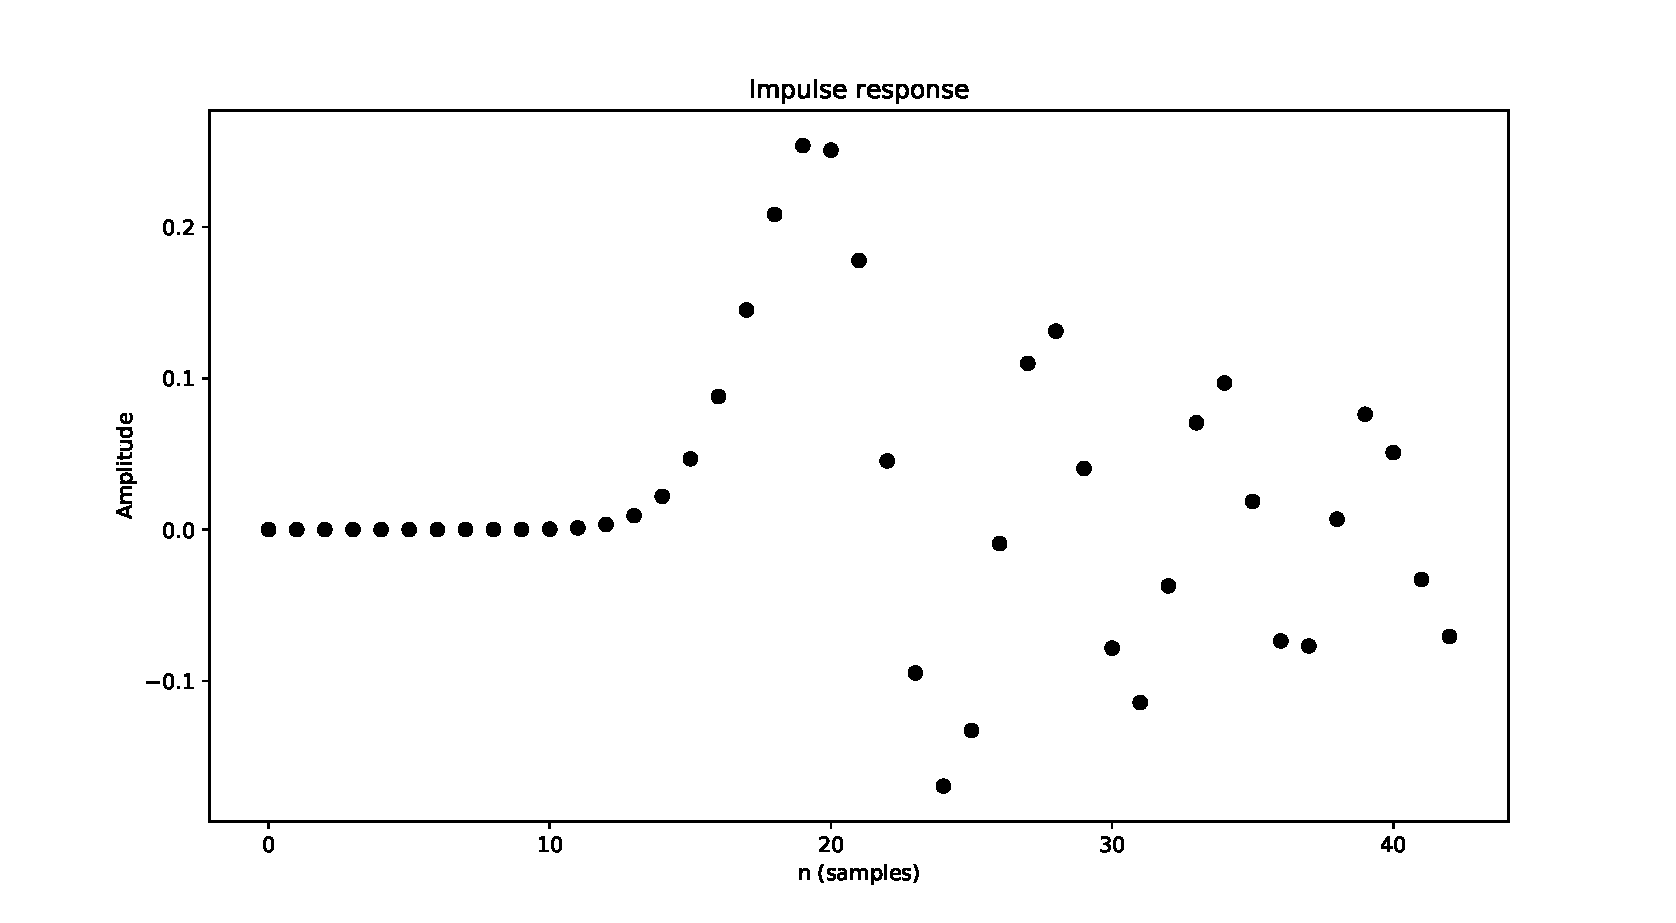
\includegraphics[scale=.4]{Figure_3.pdf}
\caption{Plotted above is the impulse response, h[n], for a Butterworth filter of low-pass type.  The y-axis indicated the coefficient value.}
\end{figure} 

Since the filter is 42nd-order, there are 42 coefficients which must be convolved with the input signal.  This order usually trends with the restrictiveness of the filter specifications.

 
\chapter{Polyphase Implementation}
\section{Multi-tap Decomposition}
\section{Relation to Direct Convolution}
\section{Hardware Implementation}
 

\end{document}